\section{D7-brane}\label{sec:D7brane}

The holographic dictionary for $N_f$ flavors of quarks in a four dimensional $SU(N)$ SYM theory is a set of $N_f$ D7-branes in the ten-dimensional supergravity dual. When $N_f << N$, it is the probe limit, meaning the additional branes do not back-react to the background geometry. 
We study the simplest setting, with only $N_f=1$ probe brane, and it wraps the warped $AdS_5$ and the three dimensional ellipsoid of the deformed $S^5$ of the Pilch-Warner metric. Furthermore, our D7-brane carries no charge, hence no worldvolume gauge field, $F = 0$. This is the equivalent setting studied in \cite{Karch:2002sh} for $AdS_5 \times S^5$, which our configuration will reduce to near the boundary, as we shall expect.


Let us consider the D7-brane embedding, whose worldvolume is induced from the target space with 
\begin{equation}\label{eq:ansatz}
 \theta = \theta(c), \quad \phi=\phi_0\equiv\frac{(2 n + 1)\pi}{2}.
\end{equation}
Consequently, the induced metric, from \eqref{eq:PWmetric} with $d\theta = \theta'(c) dc$ and $d\phi=0$, is:
\begin{align}\label{eq:PWmetric}
ds_{D7}^2 =
\Omega^2 dx_\mu dx^\mu 
- (V_c^2 +V_\theta^2 \theta'(c)^2)\, dc^2 - V_1^2 \sigma_1^2 - V_2^2 (\sigma_2^2 + \sigma_3^2).
\end{align}


%%%%%%%%%%%%%%%%%%%%%%%%%%%%%%%%%%%%%%%%%%%%%%%%%%%%%%%%%%%%%%%%%%%%%%%%%%%%%%%%%%%%%%%%%%%%%%%%%
\subsection{Action}

Our particular choice of $\phi_0$ simplifies our problem, because
\begin{equation}
 P[B_{(2)}] = 0.
\end{equation}
Then the D7-brane action is simply
\begin{align}
 S & = -T_7 \int_\mathcal{M} d^8\xi \, e^{-P[\Phi] } \sqrt{-\det g} +
 T_7\int _\mathcal{M} P[C_{(8)}].
\end{align}

Let us focus on the $C_{(8)}$ term, which was deemed as vanishing in the previous papers, \cite{Albash:2011nw} and \cite{Evans:2005ti}. The problem seemed that these authors did not consider the string frame for the metric while arguing about the Hodge star operation needed to derive $C_{(8)}$, i.e.
\begin{equation}
 dC_{(8)} = \ast dC_{(0)},
\end{equation}
in our scenario. The dilaton term from the string frame effectively cancels the vanishing factor, leading to a finite value for the pullback of the form. We decided to compute it explicitly and the full result (always up to an exact form because it is a potential), is shown in the appendix \ref{sec:backgroundFields}. We can quickly see that it is nonzero for our ansatz $\phi_0$ in \eqref{eq:ansatz}. However, $P[C_{(8)}]$ term can be much simpler, as we will see now. First, we can show that:
\begin{equation}\label{eq:C8id}
 [d C_{(8)}]_{\phi_0} = d [C_{(8)}]_{\phi_0}.
\end{equation}
The left-hand-side is simply
\begin{equation}
 [d C_{(8)}]_{\phi_0}  = \dfrac{A^2 \sin\theta \cos^3(\theta)}{\left(c^2-1\right)^2} 
\sigma_1 \wedge \sigma_2 \wedge \sigma_3 \wedge dc  \wedge dx_0 \wedge dx_1 \wedge dx_2 \wedge dx_3 \wedge d\theta,
\end{equation}
and, via \eqref{eq:C8id}, we can integrate the above expression over $\theta$ and obtain:
\begin{equation}
[C_{(8)}]_{\phi_0} = \dfrac{A^2 \cos^4\theta}{4 \left(c^2-1\right)^2} \sigma_1 \wedge \sigma_2 \wedge \sigma_3 \wedge dc \wedge dx_0 \wedge dx_1 \wedge dx_2 \wedge dx_3.
\end{equation}
The full pullback is obtained by just replacing $\theta$ by $\theta(c)$.


Now we can write the action in a more explicit way:
\begin{align}\label{eq:ActionWithTheta'}
 S = & -T_7 \int_\mathcal{M} d^8\xi \, \dfrac{A(c) \cos^3\theta (c) \sqrt{c X_1(c, \theta(c))}}{\left(c^2-1\right)^3} \sqrt{\left(c^2-1\right)^2 A(c) \, \theta '(c)^2+c} \nonumber \\
     & +T_7\int _\mathcal{M} d^8\xi \, \dfrac{A(c)^2 \cos^4\theta(c)}{4 \left(c^2-1\right)^2}.
\end{align}



%%%%%%%%%%%%%%%%%%%%%%%%%%%%%%%%%%%%%%%%%%%%%%%%%%%%%%%%%%%%%%%%%%%%%%%%%%%%%%%%%%%%%%%%%%%%%%%%%
\subsection{Kappa symmetry projector}

The kappa symmetry projector for our configuration is:
\begin{align}
\Gamma = - \dfrac{ \gamma_{(8)} \mathcal{I} }{\sqrt{-\det g}},
\end{align}
with
\begin{align}
 \gamma_{(8)} = - V_x^4 V_1 V_2^2 \Gamma_{1 2 3 4 7 8 9}( V_c \Gamma_5 +  V_{\theta} \theta'(c) \Gamma_6), 
\end{align}
where we used capital gammas to denote the gamma matrices in the local frame, see appendix \ref{sec:localframe}.

The projector can be further simplified by combining it with the chirality condition, which for mostly minus metric convention is: 
\begin{equation}
 \Gamma_{11} \epsilon = -\epsilon, \quad 
 \Gamma_{11} \equiv \Gamma_{12345678910}.
\end{equation}
Then, the supersymmetric condition \eqref{eq:susyCondition} becomes:
\begin{equation}
 \Gamma_{11} \Gamma \epsilon = \epsilon.
\end{equation}
and 
\begin{align} \label{eq:newProjector}
  \mathcal{P}' \equiv \Gamma_{11} \Gamma  = \dfrac{1}{\sqrt{1+\xi^2}}(1- i \xi  \Gamma_{510}), \quad 
   \xi \equiv  \dfrac{V_\theta}{V_c} \theta'(c),
\end{align}
where we have applied $\mathcal{I} \epsilon = -i\epsilon$ and $\Gamma_{610} \epsilon = -i \epsilon$, the latter because we can show $\mathcal{P}_- \epsilon =0$. 


%%%%%%%%%%%%%%%%%%%%%%%%%%%%%%%%%%%%%%%%%%%%%%%%%%%%%%%%%%%%%%%%%%%%%%%%%%%%%%%%%%%%%%%%%%%%%%%%%
\subsection{Supersymmetric condition}

For the Killing spinor \eqref{eq:KillingSpinor}, the invertible operator in \eqref{eq:susyCondition0} is:
\begin{align}
 \mathcal{O} &= \exp{\left(\frac{\alpha}{2}\Gamma_{56} \right)} \exp{\left(-\frac{\phi}{2}\, \Gamma_{610} \right)} \exp{\left(\frac{\beta}{2}\Gamma_{710} \mathcal{K} \right)} \\
 \mathcal{O}^{-1} &=  \exp{\left(-\frac{\beta}{2}\Gamma_{710} \mathcal{K} \right)} 
 \exp{\left(\frac{\phi}{2}\, \Gamma_{610} \right)} 
 \exp{\left(-\frac{\alpha}{2}\Gamma_{56} \right)}.
\end{align}


The kappa symmetry projector contains the operator $\mathcal{I}$, which can be replaced as follows (see notation in \ref{sec:KillingSpinor}):
\begin{equation}
 \mathcal{I}\eta =-i \eta = \Gamma_{610} \eta,
\end{equation}
where we used $\mathcal{P}_- \eta =0$ in the last step. 

Then, \eqref{eq:susyCondition0} reduces to:
\begin{equation}
 \Pi_{-} \mathcal{O}^{-1} \gamma_{(8)} \mathcal{O} \Gamma_{610} \Pi_{+}  = 0.
\end{equation}
which, after manipulating the gamma matrices, gives:
\begin{equation}
i V_1 V_2^2 V_x^4 \Pi_- \Gamma_{6 8 9 10} \mathcal{K} \sin\beta \left(V_c \sin\alpha - V_\theta \cos\alpha \, \theta'(c)\right) = 0
\end{equation}
Therefore, the condition our configuration must satisfy in order to preserve supersymmetry is:
\begin{equation}\label{eq:susyConditionTheta}
 \theta'(c) = \dfrac{V_c}{V_\theta} \tan\alpha = \dfrac{c \, \tan\theta(c)}{c^2-1} .
\end{equation}


One can repeat the analysis of \eqref{eq:susyCondition0} for the other projector $\mathcal{P}_{\pm}$, and it will give the same condition \eqref{eq:susyConditionTheta}.


The projector \eqref{eq:newProjector} at the solution \eqref{eq:susyConditionTheta} is simply
\begin{equation}
\mathcal{P}' = \cos \alpha - i \sin \alpha \, \Gamma_{510},
\end{equation}
since $ \xi =  \tan \alpha $.
No more projectors are found, therefore, ours is a 1/2-BPS embedding.

%%%%%%%%%%%%%%%%%%%%%%%%%%%%%%%%%%%%%%%%%%%%%%%%%%%%%%%%%%%%%%%%%%%%%%%%%%%%%%%%%%%%%%%%%%%%%%%%%

\subsection{Equation of motion}

As a consistency check for our results, the equation of motion from the action \eqref{eq:ActionWithTheta'} is fulfilled with the solution \eqref{eq:susyConditionTheta}. In particular, 
\begin{align}\label{eq:eom}
-\left.EL[\mathcal{L}_{DBI}]\right|_\text{solution} = EL[\mathcal{L}_{WZ}] = \dfrac{A^2 \sin\theta \cos^3(\theta)}{\left(c^2-1\right)^2},
\end{align}
where we have the Euler-Lagrange operator:
\begin{equation}
 EL[\mathcal{L}] = 
 \left(\dfrac{\pd }{\pd \theta(c)} -\dfrac{\pd }{\pd c}  \dfrac{\pd }{\pd \theta'(c)} \right) \mathcal{L}.
\end{equation}
Hence, \eqref{eq:eom} is another proof for the non-vanishing WZ term.




\subsection{Solution}

The solution to the differential equation \eqref{eq:susyConditionTheta} is:
\begin{equation}\label{eq:susyConditionSolution}
\boxed{\sin\theta(c) = L \sqrt{c^2-1}; \quad 1 < c \leq \sqrt{1+L^{-2}}, \quad L < 1},
\end{equation}
where $L$ is an integration constant, which is proportional to the mass of the fundamental matter (or quark) field in the dual field theory, as we explain next. The upper bound of $c$ is set by the maximum of the sine.

In near boundary limit, $c \approx 1 + z^2/2$, our solution reduces to the exact solution found in the $AdS_5 \times S^5$ background, see \cite{Karch:2002sh} and \cite{Karch:2005ms}, i.e.
\begin{equation}
 \sin\theta(z) = L z.
\end{equation}
As \cite{Karch:2005ms} explains, in the flat embedding space limit, this embedding describes a planar D-brane located at a constant distance away $L$ from the stack of N D3-branes:
\begin{equation}
 L = \lim_{z \rightarrow 0 } \frac{1}{z} \sin\theta(z)
\end{equation}
and this distance is proportional to the quark mass $m$:
\begin{equation}
 L = \dfrac{m}{2 \pi l_s^2}.
\end{equation}


Figures in \ref{fig:vielbeins} show the vielbeins of the induced metric at the solution, from which we learn how the geometry of the embedding looks like at different values of $c$. First, observe the divergence at $c_{max}=\sqrt{1+M^{-2}}$. This is the location of the well-known enhançon locus, at $\theta = \pi/2$, see \cite{Buchel:2000cn} and \cite{Evans:2000ct}. The spheroid is undeformed at the boundary $c=1$ and becomes squashed until it vanishes at the enhancon. 

\begin{figure}[t]
\begin{center}
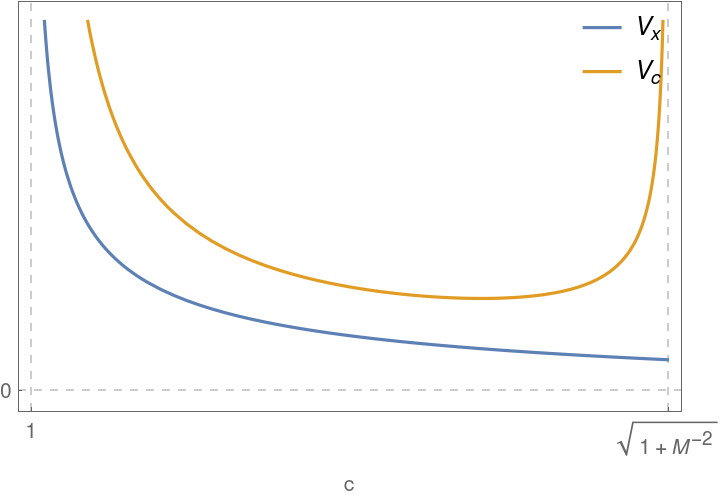
\includegraphics[width=0.6\textwidth]{pictures/vxvc.png}
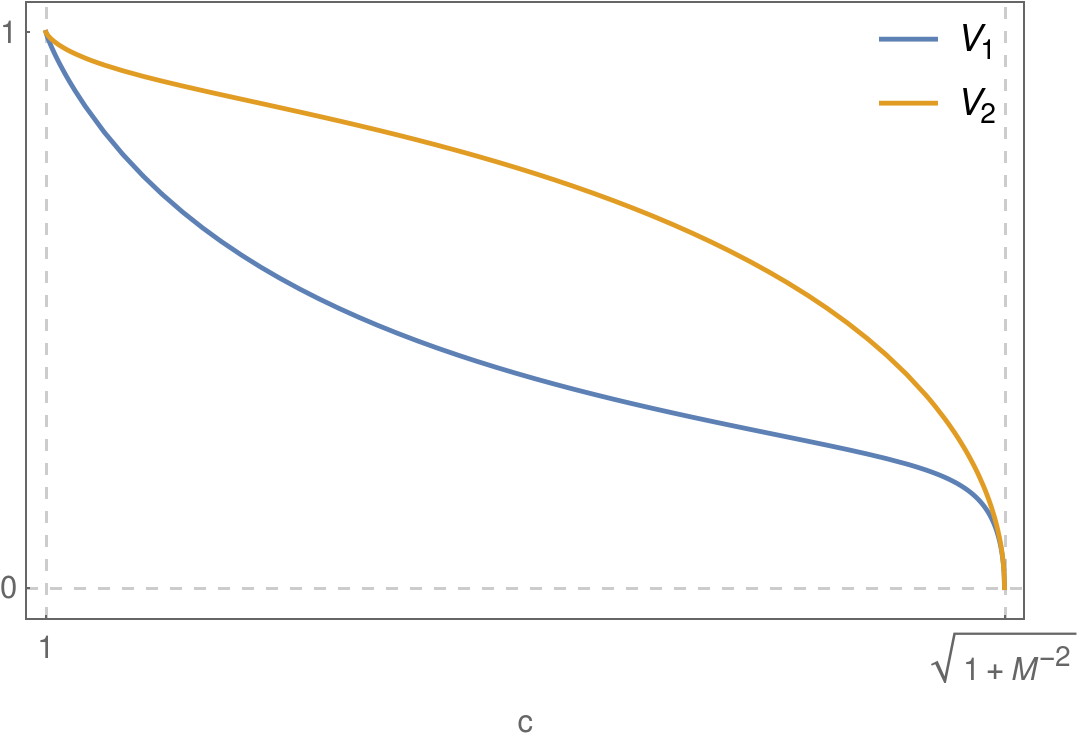
\includegraphics[width=0.6\textwidth]{pictures/v1v2.png}
\end{center}
\caption{\label{fig:vielbeins} The vielbeins of the induced metric at different values of $c$.}
\end{figure}



\subsection{Holographic renormalization}

The action evaluated at the solution \eqref{eq:susyConditionSolution} is:
\begin{align}\label{eq:ActionAtSolution}
 S = & -T_7 \int_\mathcal{M} d^8\xi \, 
 \frac{c A \left(\left(c^2-1\right) L^2-1\right) \left(c \left(c^2-1\right) L^2 A-\left(c^2-1\right) L^2+1\right)}{\left(c^2-1\right)^3}
 \nonumber \\
     & +T_7\int _\mathcal{M} d^8\xi \, 
 \frac{A^2 \left(\left(c^2-1\right) L^2-1\right)^2}{4 \left(c^2-1\right)^2},
\end{align}
where the integration of $c$ is the range shown in \eqref{eq:susyConditionSolution}.

The action is IR-divergent, as we can expect, since the boundary geometry is asymptotically AdS. The divergent terms are:
\begin{align}
 S_{IR} = T_7 \int_\mathcal{M} d^7\xi 
        \left( \frac{1}{4 \epsilon ^4} +\frac{1-L^2+\log \left(\epsilon/2\right)}{2 \epsilon ^2}-\frac{ \log ^2\left(\epsilon/2\right)}{4}+\frac{\log (\epsilon )}{8} \right).
\end{align}
The method to handle them is the holographic renormalization, and the counterterms for our action are covered by the results derived in the section 4 of \cite{Karch:2005ms}. The chiral condensate must be vanishing too, as it is prohibited by supersymmetry, \cite{Babington:2003vm}. This disagrees with \cite{Albash:2011nw}, however, as we already mentioned, their logarithmic term in the solution is incorrect, and by removing it, we recover our result and the condensate evaluated at the background is exactly the one in \cite{Karch:2005ms}, and it is zero.





